\chapter{Systembeskrivelse}
Det udviklede system består af en biomedicinsk måleopstilling med hardware- og en tilhørende softwaredel. Systemet er en invasiv blodtryksmåler udviklet til forskning. Blodtrykket skal kunne måles invasivt, således at blodtryksmålesystemet er tilsluttet et måleobjekt og kontinuerligt kan monitorere blodtrykket. 

\begin{figure}[H]
	\centering
	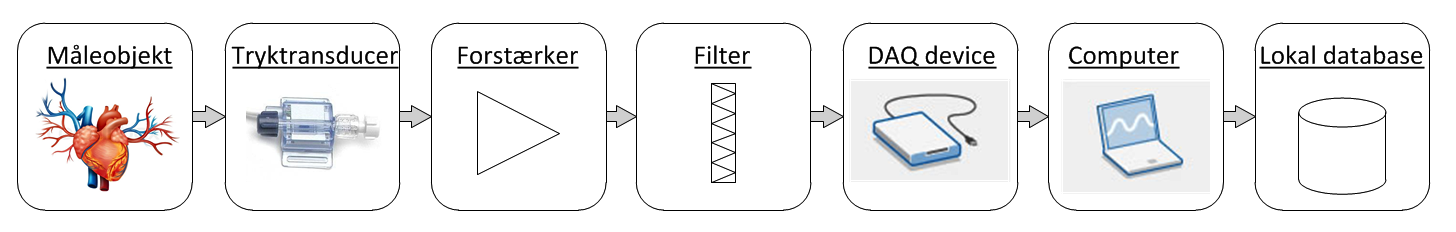
\includegraphics[width=1\textwidth]{Figurer/Snip20151209_73}
	\caption{Illustration af systemet}
\end{figure}

Den udviklede hardwaredel er opbygget som et elektrisk kredsløb, der behandler signalet. Det tryk, der ønskes behandlet kommer fra et Måleobjekt og hentes via en Tryktransducer. Tryktransduceren har til formål at konvertere Måleobjektets fysiske tryk til et analogt signal. Efter konverteringen fra tryk til et elektrisk signal forstærkes signalet i Forstærkerblokken. Forstærkningen er nødvendig, da Tryktransducerens spændingssignal er meget svagt og skal derfor forstærkes til en spænding, der er anvendelig til DAQ’en. Derudover skal signalet også filtreres i det indbyggede analoge filter, hvor signalet frasorterer frekvenser, der er højere end 50 Hz, da disse frekvenser er irrelavante for blodtrykssignalet. Når signalet har passeret Forstærker- og Filterblokken, konverteres det i DAQ’en fra det analoge signal til et digitalt signal, hvorefter signalet kan behandles af softwaren. \\\\
Systemets softwaredel er et program, der er udviklet til at vise blodtrykssignalet grafisk som funktion af tiden. Programmet er programmeret i Visual Studio C\#, og er udviklet til at være anvendelig i forskningssammenhænge. Brugergrænsefladen skal grafisk vise blodtrykssignalet kontinuert. Derudover skal Forskeren have mulighed for at optage en bestemt optagelseslængde, og derefter gemme de målte data i en lokal Database. Systemet er ligeledes opbygget til at kunne foretage en kalibrering af blodtrykssignalet. Når programmet starter, vises Kalibrerings-vinduet, hvor Forskeren har mulighed for at indtaste de målte kalibreringsdata og derefter udføre kalibreringen, hvis dette ønskes. Hvis Forsker ikke ønsker at kalibrere, skal Kalibrerings-vinduet blot lukkes, og hermed ses blodtrykssignalet grafisk i Monitor-vinduet. Monitor-vinduet giver Forskeren mulighed for at optage og  gemme en bestemt sekvens af et blodtrykssignal. Derudover giver Monitor-vinduet mulighed for at nulpunktsjustere systemet. Programmet har ligeledes et digitalt filter, som giver Forskeren mulighed for at filtrere blodtrykssignalet i selve programmet. Filteret er per default aktivt, men kan via to radiobuttons deaktiveres og aktiveres efter Forskerens ønske. 